\documentclass[review]{elsarticle}

\usepackage{lineno,hyperref}
\usepackage[brazilian]{babel}
\usepackage[utf8]{inputenc}
\usepackage{url}
\usepackage{enumitem}
\modulolinenumbers[5]
\graphicspath{ {./} }

\journal{Advanced Topics in Data Science}

%%%%%%%%%%%%%%%%%%%%%%%
%% Elsevier bibliography styles
%%%%%%%%%%%%%%%%%%%%%%%
%% To change the style, put a % in front of the second line of the current style and
%% remove the % from the second line of the style you would like to use.
%%%%%%%%%%%%%%%%%%%%%%%

%% Numbered
%\bibliographystyle{model1-num-names}

%% Numbered without titles
%\bibliographystyle{model1a-num-names}

%% Harvard
%\bibliographystyle{model2-names.bst}\biboptions{authoryear}

%% Vancouver numbered
%\usepackage{numcompress}\bibliographystyle{model3-num-names}

%% Vancouver name/year
%\usepackage{numcompress}\bibliographystyle{model4-names}\biboptions{authoryear}

%% APA style
\bibliographystyle{model5-names}\biboptions{authoryear}

%% AMA style
%\usepackage{numcompress}\bibliographystyle{model6-num-names}

%% `Elsevier LaTeX' style
\bibliographystyle{elsarticle-num}
\renewcommand{\UrlFont}{\small\tt}
%%%%%%%%%%%%%%%%%%%%%%%

\begin{document}

\begin{frontmatter}

\title{Análise do rendimento escolar em 2010}

\author{Maria Luiza Menezes Vieira}
\author{Ramon de Saboya Gomes}
\author{Ullayne Fernandes Farias de Lima}
\address{Universidade Federal de Pernambuco - Centro de Informática\\
Caixa Postal 7.851 - 50.732-970 - Recife, PE - Brasil}

\begin{abstract}
Este trabalho faz uma análise do desempenhos dos alunos no ensino básico brasileiro no ano de 2010. A análise é feita observando as taxas de aprovação, reprovação e abandono dos 9 anos do ensino fundamental e dos 4 anos do ensino médio juntamente o tipo de escola, isto é, se é pública, privada, federal etc e as zonas onde se encontram: rural ou urbana. A base de dados inclui informações de todas os municípios do país.\par
\end{abstract}

\end{frontmatter}

\linenumbers

\section{Introdução}

A qualidade da educação brasileira é um tema bastante debatido durante todos os anos, especialmente em anos de eleição, pois é muito questionado se atende os níveis esperados.\par
Segundo o IBGE \cite{G12012}, 49.3\% dos brasileiros com mais de 25 anos não possuem escolaridade ou apenas o ensino fundamental incompleto em 2010, sendo uma taxa preocupante para a qualidade dos profissionais do país, bem como a própria qualidade de vida.\par
Por este motivo, a equipe decidiu analisar o rendimento em diversos municípios, bem como validar possíveis hipóteses sobre o que aconteceu na educação brasileira naquele ano e outras relações.\par

\section{Hipóteses}
Baseados em conhecimentos populares e na criatividade da equipe diante dos conhecimentos previamente, sem pesquisas preliminares, foram levantadas quatro hipóteses sobre as taxas de rendimento e possíveis relações com os dados obtidos.\par

\subsection{Hipótese 1: O ensino médio tem o maior indice de reprovação/abandono}
A hipótese foi levantada pois acredita-se que pessoas de baixa renda precisam se afastar da escola para começar a trabalhar, dado que a família não possui condições de sustentar com a renda atual.\par

\subsection{Hipótese 2: O abandono/reprovação é maior em escolas do ensino público e em zonas rurais}
A hipótese foi levantada por um motivo similar à hipótese supracitada, acredita-se que nas zona rural os alunos precisam ajudar com a renda familiar e o problema é agravado em escolas públicas pois possuem menor suporte para os alunos.\par

\subsection{Hipótese 3: O índice de abandono está relacionado com o PIB per capita do estado}
A hipótese foi levantada pois acredita-se que o rendimento dos alunos está relacionado ao desenvolvimento do estado que ele está inserido. Por isso, será analisado se a taxa de abandono cresce na ordem inversa ao crescimento do PIB, pois quanto maior o PIB per capita de um estado, maior a possibilidade dos trabalhadores serem formais e com formação de nível superior e, para alcançá-la, é necessário concluir todo o ensino básico.\par

\subsection{Hipótese 4: As regiões norte/nordeste possuem menor nivel de aprovação que as demais regiões}
A hipótese foi levantada pois acredita-se que essas regiões possuem menos investimentos do governo, além de possuírem uma grande área onde as pessoas são segregadas, como as populações sertanejas e ribeirinhas. Dito isto, a expectativa é que a taxa de aprovação fique comprometida.\par

\section{Dados}
A análise dos rendimentos dos alunos do ensino básico do ano de 2010 foi feita utilizando a base de dados do INEP e o enriquecendo com informações sobre o PIB per capita dos municípios, estados e regiões. Inicialmente, os dados são compostos por 4 anos de análise de desempenho com objetivo de construir um acompanhamento no desempenho dos alunos pois o INEP criou um identificador único para cada, análise é possível através da adição de outras base de dados. Contudo, para o escopo deste projeto, a equipe decidiu focar em apenas um ano e observar as relações dos dados.\par

\subsection{Coleta}
Os dados utilizados neste projeto foram obtidos através da plataforma de dados do Governo Federal. Os dados originalmente foram coletados pelo INEP e a tabela utilizada analisa as taxas de rendimento em todos os municípios do país, agrupando as escolas por localização (zona urbana ou rural) e o tipo (escolas públicas, particulares, federais, estaduais e municipais).\par
O dado de PIB per capita não consta na planilha original, foi necessário o uso de uma tabela que nos desse essa informação.\par

\subsection{Pré-processamento}
As bases de dados utilizadas possuíam dados que precisavam ser corrigidos antes da análise.\par
Problemas que ocorreram em ambas as bases:\par
\begin{itemize}
    \item Nomes de Municípios errados: para corrigir o nome dos municípios, foram feitas buscas na web até conseguir atingir match entre os municípios na tabela do pib e de rendimento 
    \item Presença de pontuação: para retirar os caracteres foi aplicado uma substituição simples usando uma normalização da biblioteca unicodedata, que substituiu os caracteres acentuados pelos equivalentes sem acento da tabela ASCII. 
\end{itemize}
Um dos problemas encontrados foi um caso de um bairro que estava listado na base de dados como um município, por isso, foi removido. Além disso, foi a sincronização dos nomes dos municípios em ambas as bases, por exemplo, o município de Barro Preto, que estava listado com seu nome antigo (Governador Lomanto Júnior).\par
Para fazer o enriquecimento da base de rendimento foi feito um processo de associação do PIB per capita dos municípios, gerando uma nova coluna no \emph{dataframe} de municípios com o valor do mesmo.
Além do tratamento dos dados já comentando, a escala dos dados também se tornou um incômodo porque o pib e as taxas estavam em escalas diferentes o que foi prejudicial nas análises. Para resolver isto, os dados foram normalizados onde cada elemento de uma coluna era subtraído do menor valor e dividido pela amplitude.\par

\section{Análise dos dados}
Nesta etapa do projeto foi feita a análise dos dados com objetivo de verificar a validade das hipóteses levantadas pela equipe com objetivo de entender melhor o comportamento dos rendimentos dos alunos de 2010. Será discutido o modo de validação de cada hipótese, além do agrupamento dos dados realizado.\par

\subsection{Metodologia de validação}

\subsubsection{Hipótese 1}
A validação da hipótese 1 através de análise do comportamento da taxa de aprovados porque a soma da taxa de aprovados, reprovados e abandonos é igual a 100, portanto foi feita a análise do complemento da hipótese. Para isso, foram adicionadas as médias de aprovações do ensino médio e no ensino fundamental foi separado nos intervalos de 1:5 (primeiro ao quinto ano) e 6:9 (sexto ao nono ano) como é possível observar na tabela ~\ref{fig:t1}.\par
\begin{figure}[h!]
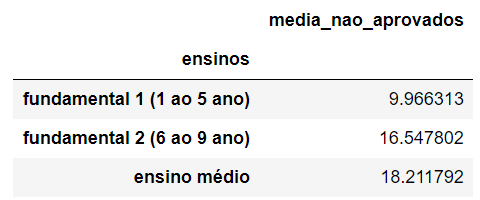
\includegraphics[width=250pt]{h1_table.png}
\caption{Tabela 1}
\label{fig:t1}
\centering
\end{figure}

\subsubsection{Hipótese 2}
A validação da hipótese 2 foi feita agrupando as informações de não aprovados, como feito na hipótese anterior, i.e, junção da taxa de reprovados e de abandono. A informação agrupada foi indexada pelo par de localização e rede, com um total de 10 combinações (\{Rural, Urbana\} X \{Particular, Público, Federal, Estadual, Municipal\}) como na tabela ~\ref{fig:t2}.\par
\begin{figure}[h!]
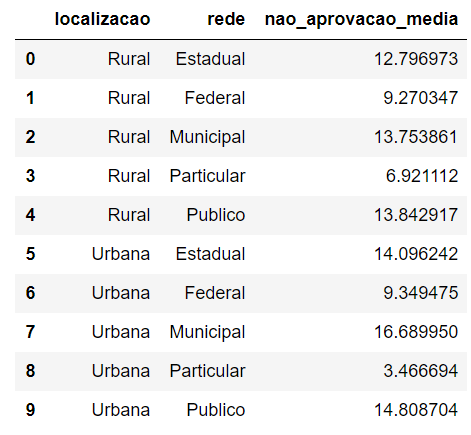
\includegraphics[width=300pt]{h2_table.png}
\caption{Tabela 2}
\label{fig:t2}
\centering
\end{figure}

\subsubsection{Hipótese 3}
A validação da hipótese 3 foi realizada através da análise do comportamento entre a tendência de crescimento do pib com as variações de cada ano do ensino básico. Na hipótese, inicialmente, seria considerado o pib dos estados porém acredita-se que seria perda de informação não levar em consideração a variação do pib do município igualmente. Por este motivo, esta hipótese teve duas soluções, mas com abordagens distintas.\par
A análise feita para observar a relação entre o pib do município e as séries do ensino básico utilizou o coeficiente de \emph{Pearson} e o coeficiente de \emph{Spearman} para buscar a correlação entre as variáveis. Primeiramente, para cada série do ensino básico foi calculado a relação com o pib utilizando o \emph{Pearson}, contudo os resultados foram todos bastante próximos de zero. Por este motivo, foi-se necessário aplicar outro método de correlação de variáveis, pois poderia haver alguma relação entre os dados e o PIB que não fosse linear e isso foi resolvido com o coeficiente de \emph{Spearman} que busca correlações que podem não ser linear.\par
A análise que relaciona o pib dos estados com as taxas de abandono das séries utilizou uma abordagem diferente pois agrupou os dados por: aprovados, reprovados e abandonos e comparou com o pib per capita do estado. É possível observar as relações no heatmap que relaciona as taxas de abandono com o pib de cada estado.\par

\subsubsection{Hipótese 4}
A validação da hipótese 4 foi feita pelo agrupamento dos valores das taxas de aprovação dos municípios das 5 regiões. Com essa informação agrupada pela média, é possível realizar a comparação entre as regiões.\par

\subsection{Agrupamento dos dados}
Além da análise dos dados realizada para validação das hipóteses, a equipe utilizou um algoritmo de agrupamento de dados a fim de observar outras possíveis relações que pudessem existir nos dados. Para agrupar os dados, foi utilizado o algoritmo \emph{k-means}, que busca formar \emph{k} grupos com algum nível de similaridade. Com objetivo de observar se as regiões possuíam comportamentos parecidos, foi o \emph{k-means} foi configurado para agrupar 5 grupos.\par
Para cada grupo retornado pelo algoritmo, foi analisado: 
\begin{itemize}[noitemsep]
    \item As regiões que estavam presentes.
    \item Redes: {Pública, privada, federal, municipal}
    \item Localização: {Zona rural, Zona urbana}
    \item Para cada região, em cada grupo, as taxas de: aprovados, reprovados e abandonos 
\end{itemize}
Estas análises buscavam observar o padrão do agrupamento dos dados. Para fazer esta análise, foram retiradas dos dados categóricos da base de dados e adicionados posteriormente, pois sua presença prejudicava o algoritmo \emph{k-means}. 

\section{Resultados}

Para a hipótese 1, percebemos que de fato o ensino médio possui a maior taxa de reprovação/abandono, tornando a hipótese validada, porém a diferença mais significativa é entre o ensino fundamental 1 e o ensino fundamental 2 como observado no gráfico abaixo Quando buscamos informações sobre o trabalho infantil, encontramos, por exemplo uma pesquisa do IBGE de 2015 \cite{OGLOBO16} em que 44,2\% dos brasileiros ocupados tinham começado a trabalhar antes dos 14 anos. Mesmo sendo de um ano diferente, a informação verifica o fato observado, pois a faixa etária do ensino fundamental 2 vai de 11 a 15 anos, como visto na figura ~\ref{fig:h1}.\par
\begin{figure}[h!]
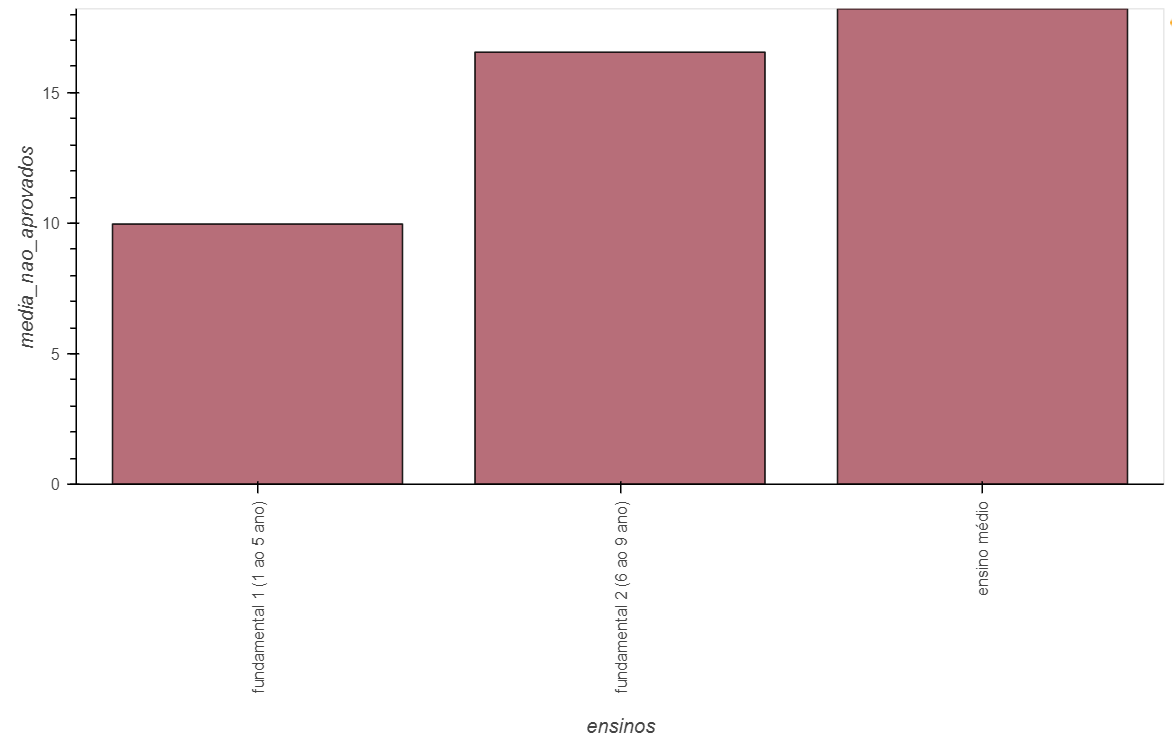
\includegraphics[width=300pt]{h1_graph.png}
\caption{Hipótese 1}
\label{fig:h1}
\centering
\end{figure}
Já em relação à hipótese 2, foi possível perceber que, independente de zona, as escolas particulares de fato tem as menores taxas de reprovação entre todas as modalidades, porém, ao levarmos as zonas em consideração percebemos que a zona urbana possui as maiores reprovações em todos os tipos de escolas, exceto entre as particulares. Esta hipótese foi, por tanto, parcialmente validada.\par
\begin{figure}[h!]
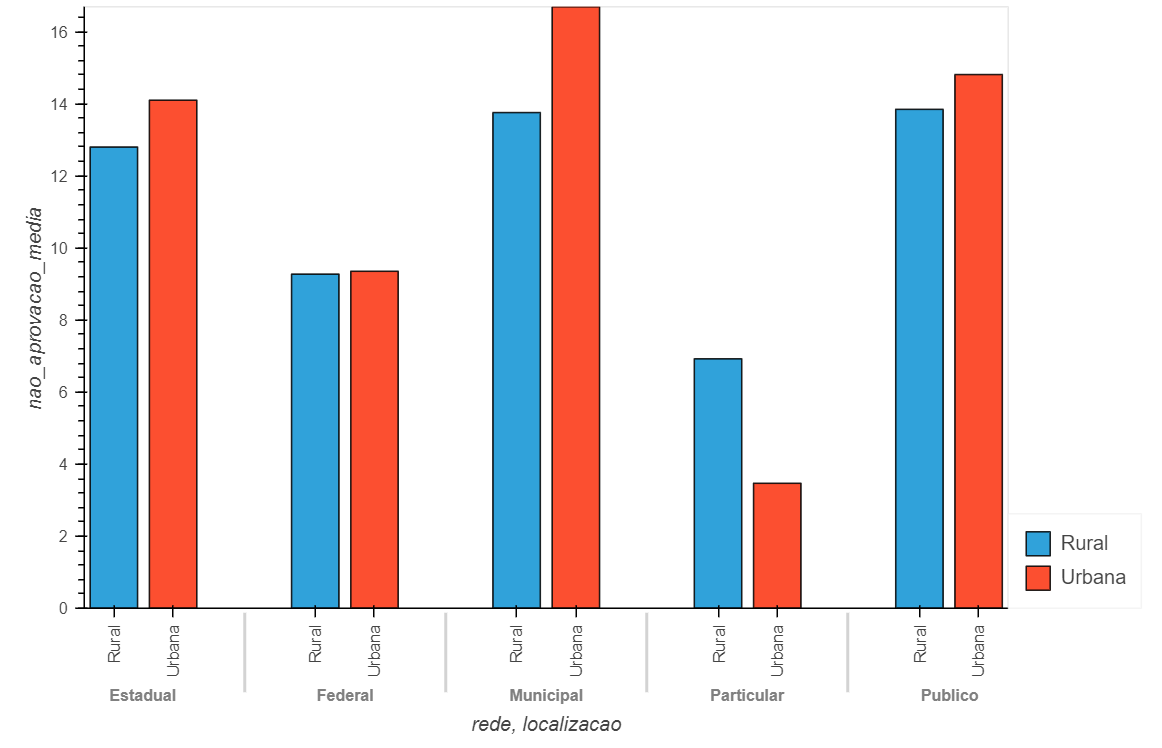
\includegraphics[width=300pt]{h2_graph.png}
\caption{Hipótese 2}
\label{fig:h2}
\centering
\end{figure}
A hipótese 3 comenta de uma possível relação inversamente proporcional do PIB per capita de um estado com sua taxa de abandono e através do \emph{heatmap} (figura ~\ref{fig:h3}), podemos observar que há uma relação inversa, porém não necessariamente linear.\par
\begin{figure}[h!]
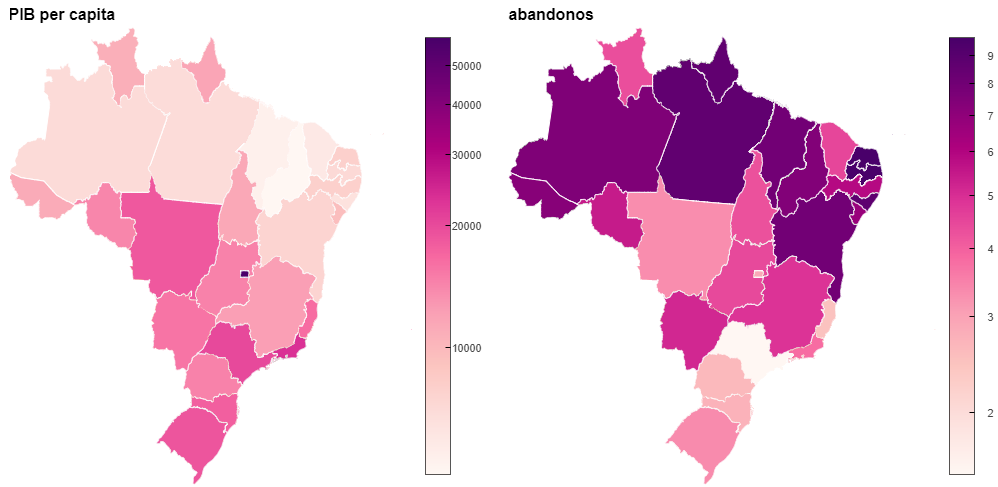
\includegraphics[width=350pt]{h3_graph.png}
\caption{Hipótese 3}
\label{fig:h3}
\centering
\end{figure}
Quando a granularidade é aumentada e é feita a análise através do PIB do município, entretanto, é possível observar através do coeficiente de \emph{Pearson} que não há relação linear com a taxa de abandono, apesar de existir com alguma relação não linear, como mostrada por \emph{Spearman}. Após a correlação de \emph{Spearman}, foi possível observar que existe relação de alguns das séries com o pib como é possível observar com os valores de \emph{pvalue} retornados pelo método de \emph{Spearman}.  Os valores retornados estão muito próximos a zero, o que implica que exclui a possibilidade de não existir correlação entre os valores das séries e o pib dos municípios. Contudo, é possível observar no gráfico (figura ~\ref{fig:h31}) que relaciona a taxa de abandono com o pib dos municípios que grande parte dos dados se concentram no próximo à origem do plano cartesiano, mostrando que mesmo que haja uma relação, a relação não é forte o suficiente para ser expressiva.\par
\begin{figure}[h!]
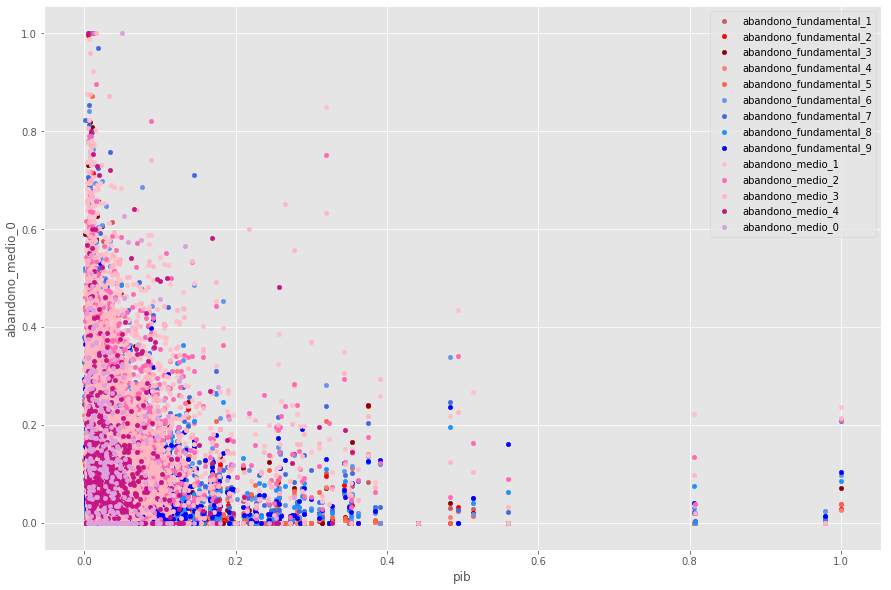
\includegraphics[width=350pt]{h3_scatter.png}
\caption{Hipótese 3}
\label{fig:h31}
\centering
\end{figure}
Para a última hipótese, observou-se (figura ~\ref{fig:h4}) que, de fato, as regiões Norte e Nordeste ficam abaixo das demais regiões em relação às taxas de aprovação, inclusive ficando abaixo da média entre todas elas.\par
\begin{figure}[h!]
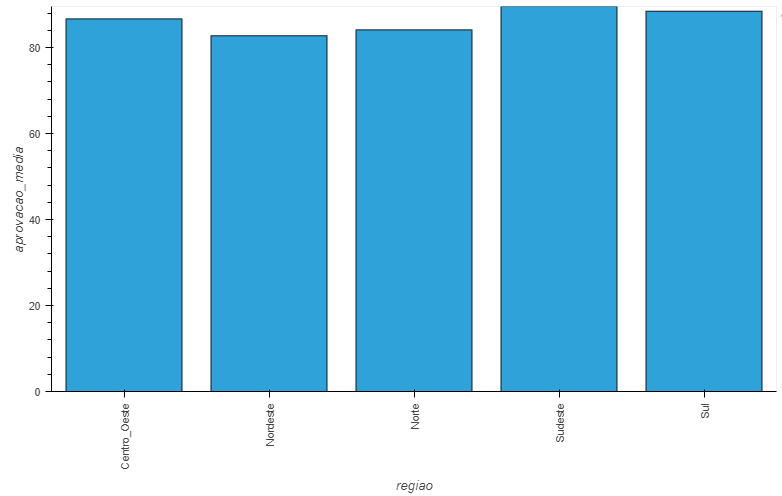
\includegraphics[width=300pt]{h4_graph.png}
\caption{Hipótese 4}
\label{fig:h4}
\centering
\end{figure}
A clusterização dos dados resultou em 5 clusters que foram analisados pelos grupos categóricos. Inicialmente, observou se as regiões tinham comportamentos parecidos. (figura ~\ref{fig:c1})\par
\begin{figure}[h!]
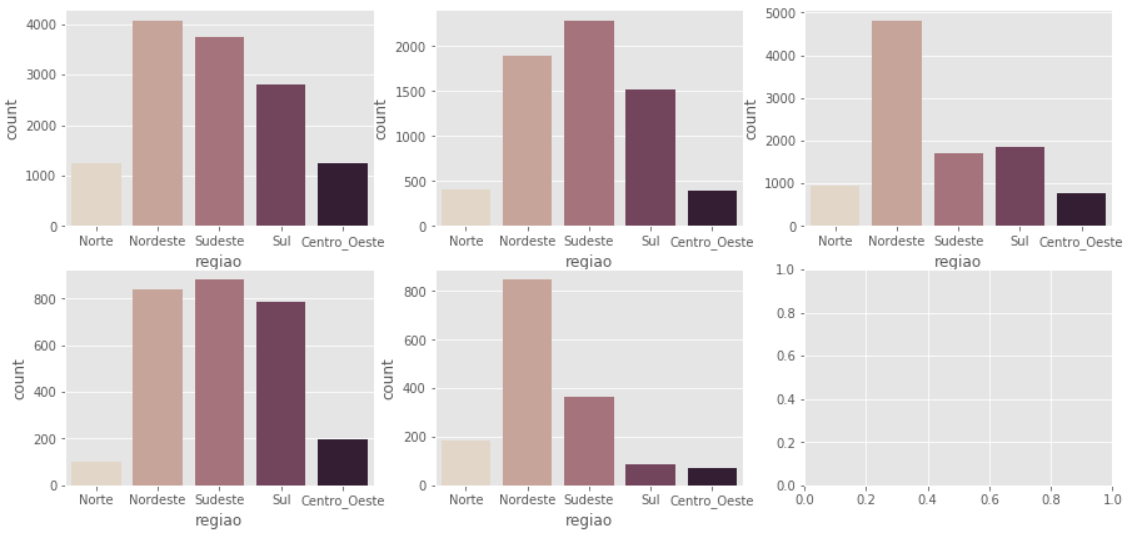
\includegraphics[width=345pt]{cluster_1.png}
\caption{Agrupamento}
\label{fig:c1}
\centering
\end{figure}
Contudo, é possível observar a presença das cinco regiões em cada cluster, o que mostra que as regiões não possuem padrões parecidos de comportamento em relação ao rendimento acadêmico dos alunos.\par
Após a análise das regiões, observou-se (figura ~\ref{fig:c2}) a disposição das redes em cada cluster.\par
\begin{figure}[h!]
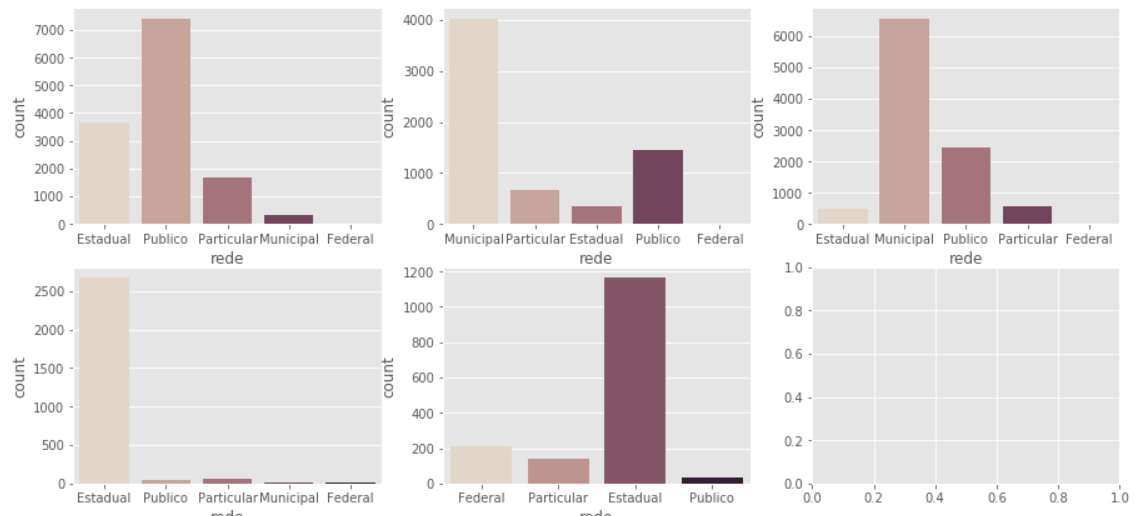
\includegraphics[width=345pt]{cluster_2.png}
\caption{Agrupamento}
\label{fig:c2}
\centering
\end{figure}
É possível observar que as redes sim possuem comportamentos parecidos que foram evidenciados nos clusters, como é possível notar na imagem de baixo mais a esquerda onde  a presença de "Estadual" é quase unanimidade. Após analisar o comportamento da rede, o último atributo categórico relevante é a localização da escola. (figura ~\ref{fig:c3})\par
\begin{figure}[h!]
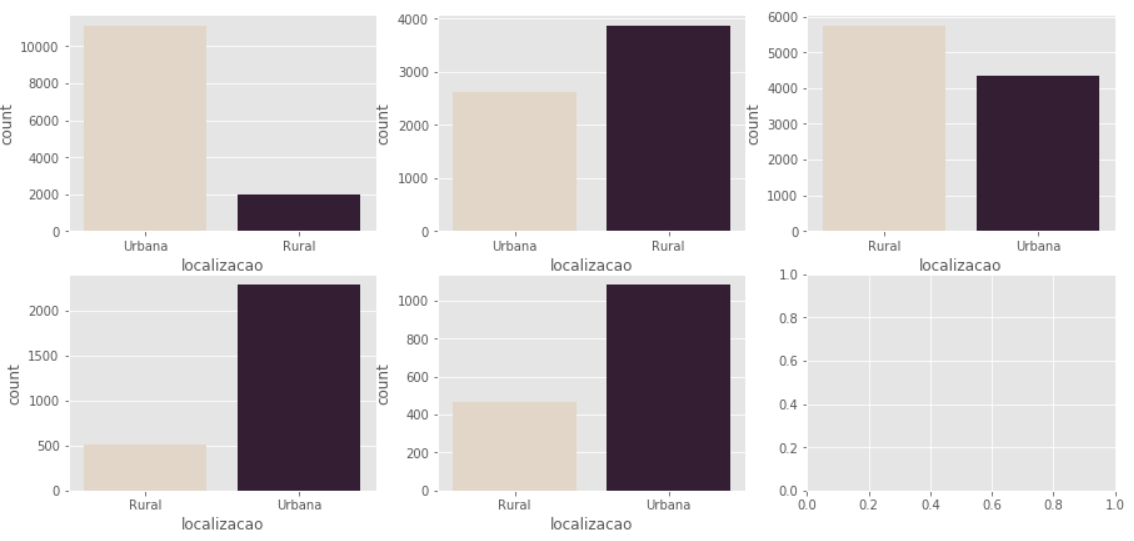
\includegraphics[width=345pt]{cluster_3.png}
\caption{Agrupamento}
\label{fig:c3}
\centering
\end{figure}
A qual se destacou em alguns casos com comportamentos parecidos. Por fim, observou-se também o desempenho, em cada cluster, das taxas de aprovação, reprovação e abandono agrupadas por região, pois foi a premissa do algoritmo de clusterização. (figura ~\ref{fig:c4})\par
\begin{figure}[h!]
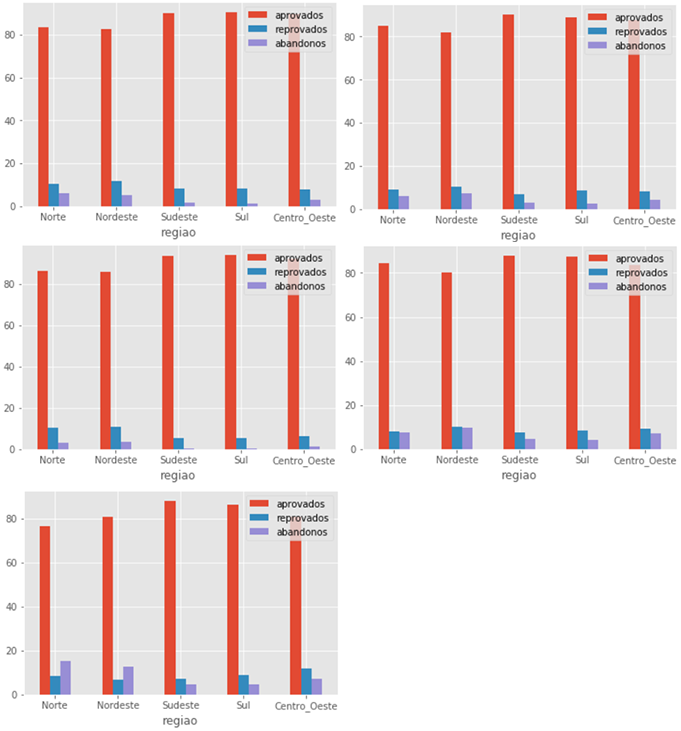
\includegraphics[width=345pt]{cluster_4.png}
\caption{Agrupamento}
\label{fig:c4}
\centering
\end{figure}
Após observar o desempenho relativo a cada região nos clusters é possível notar que, de fato, norte e nordeste possuem a taxa de aprovação menor que as demais e que de um cluster para outro a variação desses valores foi baixa o que leva a entender que região, taxa de abandono, reprovação e aprovação nao sao suficientes para observar um padrão de comportamento, contudo redes e localização possuem chances maiores de serem considerados bons atributos para seleção de padrões. Este fato pode ser explicado por materias como \cite{UOL2012, G12011}. 

\section{Conclusão}

Este trabalho permitiu a equipe romper com alguns preconceitos, mas também buscar entender por quê eles existiam e por quê o comportamento se deu de determinada forma.
Percebemos que, de fato, existem condições mais favoráveis à conclusão do ensino básico e possível ingresso ao ensino superior e mercado de trabalho formal, gerando questionamentos para além da pesquisa realizada, e envolvendo também nossa percepção social do contexto do país.

\section{Trabalhos futuros}
\begin{itemize}
    \item Aprofundar sobre os anos que possuem maior abandono/reprovação, bem como fazer uma análise ao longo do tempo.
    \item Analisar como se comportam as zonas urbanas e rurais em relação ao desempenho, desconsiderando o tipo da escola usado na hipótese. 
    \item Gerar clusters que indiquem os perfis que indiquem as condições para melhor desempenho
    \item Buscar dados sobre a Prova Brasil e avaliar a relação da mesma com o rendimento das escolas.
\end{itemize}

\section*{References}
\bibliography{bibliography}

\end{document}